\documentclass[master=ebin,english,oneside,font=lm]{kulemt}
\setup{title={Global-to-Local Segmentation and Genotypic Analysis of Brain Shape Asymmetry},author={Vasileios Lemonidis},promoter={Prof. Peter Claes\\ Dept. of Electrical Engineering\\ Dept. of Human Genetics \\~\\ Prof. Isabelle Cleynen \and Dept. of Human Genetics}, assessor={Asst. Prof. Rose Bruffaerts\\ Dept. of Biomedical Sciences\\ University of Antwerp\\~\\  Prof. Lieve Moons \and Dept. of Biology} ,assistant={MSc. Meng Yuan \and MSc. Seppe Goovaerts},acyear=2022,bind=3mm,inputenc=utf8}


\usepackage[table]{xcolor} % for cell colors
\usepackage{changepage,threeparttable}
\usepackage{svg}
\usepackage{booktabs}
\usepackage{tabularx}
\usepackage{wrapfig}
\newcolumntype{Y}{>{\centering\arraybackslash}X}
\usepackage{makecell}
\usepackage{adjustbox}
\usepackage[pdfusetitle,hidelinks,plainpages=false]{hyperref}
\usepackage{algorithm}
\usepackage[noend]{algpseudocode}
\usepackage[font=small,labelfont=bf]{caption}
\usepackage{subfig}
\usepackage{changepage}
\usepackage{multirow} % for borders and merged ranges
\usepackage{soul}% for underlines
\usepackage[numbers]{natbib}
\bibliographystyle{abbrvnat-maxbibnames10}
\pdfminorversion=7
\pdfsuppresswarningpagegroup=1
%\bibliographystyle{plainnat-maxbibnames10}

\graphicspath{
	{../results},
	 {graphics}
}
\usepackage{acro}
\acsetup{
	make-links = true , % boolean
	list/display=all,
	subsequent-style =short
	}
\DeclareAcronym{gwas}{
short=GWAS,
long=genome wide association studies
}
\DeclareAcronym{mvgwas}{
short=mvGWAS,
long=multivariate genome-wide association study}
\DeclareAcronym{da}{
	short=DA,
	long=directional asymmetry
}
\DeclareAcronym{mri}{
short=MRI,
long=magnetic resonance imaging
}

\DeclareAcronym{snp}{
	short=SNP,
	long=single nucleotide polymorphism}
\DeclareAcronym{hsc}{
	short=HSC,
	long=hierarchical spectral clustering}
\DeclareAcronym{cca}{
	short=CCA,
	long=canonical correlation analysis}
\DeclareAcronym{ld}{
	short=LD,
	long=linkage disequilibrium}
\DeclareAcronym{fa}{
	short=FA,
	long=fluctuating asymmetry}
\DeclareAcronym{anova}{
short=ANOVA,
long=analysis of variance}
\DeclareAcronym{rss}{
short=RSS,
long=residual sum of squares}
\DeclareAcronym{dof}{
short=DOF,
long=degree of freedom,
short-plural=s,
long-plural-form=degrees of freedom}
\DeclareAcronym{dna}{
	short=DNA,
long=deoxyribonucleic acid}
\DeclareAcronym{rna}{
	short=RNA,
	long=ribonucleic acid}

\DeclareAcronym{cns}{
short=CNS,
long=central neural network
}
\DeclareAcronym{rc}{
short=R-C,
long=rostral-caudal}
\DeclareAcronym{dv}{
short=D-V,
long=dorsal-ventral}
\DeclareAcronym{lr}{
	short=L-R,
long=left-right}
\DeclareAcronym{rgc}{
short=RGC,
long=radial glial cell,
short-plural=s,
long-plural=s
}
\DeclareAcronym{npc}{
short=NPC,
long=neuroepithelial cell,
short-plural=s,
long-plural=s}
\DeclareAcronym{3d}{
short=3D,
long=three-dimensional}
\DeclareAcronym{dk}{short=DK,long=Desikan-Killiany}
\DeclareAcronym{adhd}{short=ADHD,long=attention-deficit / hyperactivity-disorder}
\DeclareAcronym{gpa}{short=GPA, long=generalized Procrustes analysis}
\DeclareAcronym{maf}{short=MAF, long=minor allele frequency}
\DeclareAcronym{tf}{short=TF, long=transcription factor}
\DeclareAcronym{glm}{short=GLM, long=generalized linear model}
\DeclareAcronym{fdr}{short=FDR, long=false discovery rate}
\DeclareAcronym{ml}{short=ML, long=machine learning}

\makeatletter\AtBeginDocument{\let\@elt\relax}\makeatother

\makeatletter
\renewcommand{\cleardoublepage}{\clearpage \ifodd\c@page\else
	\hbox{}\newpage\if@twocolumn\hbox{}\newpage\fi\fi}
\makeatother

\usepackage{amsmath}
\DeclareMathOperator*{\argmax}{arg\,max}
\DeclareMathOperator*{\argmin}{arg\,min}
\DeclareMathOperator*{\erfc}{erfc}
\DeclareMathOperator*{\NMI}{NMI}
\begin{document}
\newenvironment{acknowledgements}%
{\cleardoublepage\thispagestyle{empty}\null\vfill\begin{center}%
		\bfseries Acknowledgements\end{center}}%
{\vfill\null}
\begin{acknowledgements}
	I would like to convey my deep gratitude to everyone that  supported me throughout the writing of this thesis. Specifically, professor Peter Claes provided the grounds for its conception and a concrete plan for its manifestation, offering me access to the essential tools, data and advice. Professor Isabelle Cleynen supplied me with the necessary threoretical basis on population genetics, without which I would not be capable or feel confident enough to confront the thesis' complexity. My mentors, PhD students Meng Yuan and Seppe Goovaerts, offered extremely valuable feedback through frequent communication and to-the-point advice at every step of the project, successfully guiding me towards its realization. Last but not least, I owe a great thank you to the people that stood beside me, family and friends, whose tolerance and support comprised the cornerstone of this effort.
\end{acknowledgements}
\tableofcontents*
\cleardoublepage
\listoffigures
\listoftables
\cleardoublepage
\addcontentsline{toc}{chapter}{List of Abbreviations}
\printacronyms[name=Abbreviations]
\begin{abstract}
	The overall purpose of this thesis has been to complement the existing bibliography on the detection and examination of the genetic associations of brain shape asymmetry. Asymmetry components  are computed based on the  brain \ac{mri} dataset provided by UK Biobank database. A data-driven approach is followed, where the brain surface is partitioned in an unsupervised manner, through  \ac{hsc}, a technique that allows for  a coarse-to-fine segmentation. Aggregated asymmetry measurements are retrieved from the segments, whose genetic association is examined through a \ac{mvgwas} statistical analysis. Recognized significant \acp{snp} were then analyzed individually or in groups, through comparison with existing results and databases.  The genetic overlap with neurodevelopmental disorders and traits, that have been reported to exhibit phenotypic associations with brain structure asymmetry, such as autism, Alzheimer’s disease or intelligence, were examined. Functional annotations of variants associated with the genes where significant \acp{snp} were detected were obtained, offering an insight into the functional reasoning behind the brain shape asymmetry existence.
\end{abstract}
\acresetall
\mainmatter
\chapter{Introduction}
\label{chap:introduction}

\section{Bilateria lineage}
Cerebral bilateral symmetry is a universal quality of organisms belonging to the Bilateria lineage \cite{Concha2012}\cite{Corballis2009}, the phylum incorporating all species with a single plane of symmetry, in contrast with their sister group, Cnidaria (\autoref{fig:bilateriaphylum}). Bilateral symmetry is a byproduct of the activity of two separate developmental processes, that produce two axes of polarity \cite{Finnerty2003}, and therefore a symmetry plane; the formation of a primary body axis, that corresponds to the long anatomical dimension of the animal, called \acf{rc} (i.e. head-to-tail), primarily dictated by highly conserved controlled activation of HOX genes during cell differentiation; the shaping of a secondary body axis, orthogonal to \ac{rc}, named \acf{dv} (i.e. back-to-front), attributed to a variety of genes,  such as the chromatin organizer CTCF, the left-right determination factor Nodal and central HOX genes \cite{Heger2020}.  For the mammals group, the brain is anatomically divided into a left and right hemisphere.  Another important bilateria common characteristic is the germ line \textbf{triploblasticity}: the embryo begins as a flat disk with three distinct cell layers called \textbf{endoderm}, \textbf{mesoderm}, and \textbf{ectoderm}. Of significance in the neural system formation is the ectoderm, which is initially equivalent to one of the flat disk sides. Shortly after conception, the disk folds, in a way that the ectoderm side forms a tube-like shape, named \textbf{neural tube}, which acts as the neural system precursor, under a process called \textbf{neurulation}. All bilateria exhibit a \ac{cns}, which entirely develops from the neural tube walls \cite{F.Bear2016a}. Next pivotal step in the brain development, \textbf{differentiation}, leads to the creation of three distinct compartments along \acf{rc} axis, the \textbf{forebrain}, which develops into the brain cerebellum, the \textbf{midbrain}, and the \textbf{hindbrain}, which gives rise to the spinal cord in vertebrates. Until this stage, perfect bilateral symmetry is observed in the \ac{cns}. [CITATION NEEDED] Because of the highly diverse mechanisms acting on bilateria subgroups after this developmental step of \ac{cns},  the focus is subsequently directed on the vertebrates case. 


\section{Neurogenesis}
The cells comprising the neural tube are named \textbf{neuroepithelial}, and exhibit similar properties with stem cells, that is limited multipotency (i.e. they can differentiate into multiple cell types) and limited self-renewing (i.e. they can divide symmetrically into new neuroepithelial cells a finite number of times) \cite{Gotz2005}, while also properties of epithelial cells, that is polarity (i.e. asymmetrical cellular organization, with distinct basal and apical surfaces) and attachment (i.e. junctions connect adjacent cells) . After anatomical differentiation, self-renewing is activated, leading to cells proliferation and \ac{cns} bilateral expansion, while attachment is hindered, gradually exchanging the neuroepithelial cells with \textbf{radial glial (RG) cells}, the fate-restricted progenitors of neurons, marking the initiation of \textbf{neurogenesis}.\cite{Gotz2005}

Among a set of common properties, a

At the early developmental stages, the brain precursor





 



Phenomena, such as the asymmetric cell division of neuroblasts for the proteostoma case and of radial glial cells for the vertebrate case \cite{Bailly2013} , or the neuroblasts (i.e. neural stem cells) unilateral programmed migration  in vertebrates, asymmetric fluid flow   by motile cilia-generated hair-like i.e. cell organelles with the ability to beat) \cite{Grimes2017}, generate a solid basis for asymmetry presence in the \ac{cns}, implying different cell ratios of similar types on each \ac{dv} side \cite{Concha2012}. Cerebral bilateral symmetry therefore begins breaking down during fetal development, with the results in humans being anatomically visible (\autoref{fig:brainlat}). This fact gives rise to partial functional disassociation, called brain lateralization, the differential activation of each hemisphere for subsets of tasks. Lateralization becomes visible when examining organisms' behavior, with the most studied trait in humans being handedness and language \cite{Schmitz2019}\cite{Corballis2009}. 
Along with the purely genetic reasons, environment also plays a significant role in affecting cerebral bilateral asymmetry. How the environmental effect manifests itself though differs across species, with the primary reason being that neurogeneration is quite limited in humans during adulthood, with a high percentage of neuroblasts unable to migrate long distances or survive, a case that does not hold, for example, for rodents \cite{Ernst2015}. There has  


\begin{figure}
	\centering
	\includegraphics[width=0.7\linewidth]{bilateria_phylum}
	\caption[Bilateria clade \cite{Hejnol2016}]{Species phylogenetic tree subset, displaying bilateria clade, its sister clade, Cnidaria, and the direct children\cite{Hejnol2016}. Of great importance on the evolutionary studies of bilateral symmetry is the Xenacoelomorpha clade.}
	\label{fig:bilateriaphylum}
\end{figure}

\begin{figure}
	\centering
	\includesvg[width=\textwidth]{da_visualization}\\
	\caption[Illustration of brain asymmetry]{Illustration of brain asymmetry. Normalized differences of the distances of landmarks from the center of mass of each averaged hemisphere midthickness surface, after a scaling and alignment process, across the studied population.}
	\label{fig:brainlat}
\end{figure}

\section{Phenotypic trait analysis}
\subsection{Summary on cortex anatomy}
 
\subsection{Dataset Description}
 
\subsection{Shapes Normalization}
\Ac{mri} output is affected by the subject positioning and technical error.  Volumetric differences also increase the level of discrepancies among \ac{mri} samples. To remedy positioning and volume deviations, a normalization is required, achieved by projecting each subject onto \textbf{Kendall shape space} \cite{Klingenberg2020}. TO BE CONTINUED

 
\subsection{Asymmetry Components}
TO BE CONTINUED
Of primary interest in this work is \ac{da}, the asymmetric component that arises by comparing a single individual's hemispheric surfaces landmarks differences, computed through a process of alignment, reflection and subtraction of the landmarks pairs. \ac{da} captures information about anatomic characteristics, such as the overall counterclockwise torque, named `Yakovlevian torque' \cite{LeMay1976}, that is observed in humans between the right and left hemisphere (\autoref{fig:yaktorque}). Past studies have shown that abnormal \ac{da} may be an indication of certain diseases. The lack of it may imply schizophrenia predisposition \cite{Ribolsi2014}. Any significant abnormalities may be indicative of other psychiatric disorders, such as autism or developmental language disorder \cite{Herbert2005}\cite{Kong2022}. 

\subsubsection{Statistical analysis}
Bilateral asymmetry is mainly described using three components in literature \cite{klingenberg2002}\cite{Vingerhoets2021}; \acf{da}, the focus of this study, corresponds to the hemispheric side effect; antisymmetry, which is related to the effect where sidedness is random in a population (i.e. left-right randomly switches to right-left), is not observed in the human cerebral cortex, in contrast to other internal organs positions, or organisms \cite{Neubauer2020}; \acf{fa}, encompasses any random developmental and environmental effects, that cannot be explained with the existing knowledge. The observed deviations can be statistically linearly modeled as products of two effects, the hemisphere side studied and the individual specimen analyzed, as well as their interaction \cite{klingenberg2002}. Formally, based on \cite{VanDongen1999} assuming the presence of replications of the observation per individual, to account for technical error, a mixed linear model representing the aforementioned dependencies is defined as:
\begin{equation}
	Y_{ijk} = \mu + \beta + I_i + S_{ij} + E_{ijk}
\end{equation}
where $Y_{ijk}$ is the phenotype of the i-th individual, from the j-th side, under the k-th replication, $\mu$ and $\beta$ are the fixed intercept and fixed side effect respectively, $I_i\sim\mathcal{N}(0,\sigma^2_{ind})$ is the random individual effect,  $S_{ij}\sim\mathcal{N}(0,\sigma^2_{FA})$ is the random side and individual specific effect, matched to \ac{fa}, and $E_{ijk}\sim\mathcal{N}(0,\sigma^2_{ME})$ is the measurement error. Replications are necessary in such a study, in order to differentiate \ac{fa} effect from the measurement error. Given this definition, a way to measure the statistical significance is through an F-test applied on 2-way \ac{anova}, to relate the \ac{rss} ratios of effects to observable error terms, and of fluctuating effect to the measurement error. Extra care needs to be given on the determination of the \ac{dof} of each term, given the preprocessing applied to bring the hemispheres surfaces into Kendall shape space. Those are extracted from the rigorous work in \cite{klingenberg2002}. Given that the analysis is performed on a pair of symmetric objects, and not on a single symmetric object, this configuration is named matching asymmetry analysis. In order to avoid further de facto assumptions, regarding the distribution of TO BE CONTINUED
\subsection{Phenotypic partitioning}\label{sec:hsc}
\Acf{hsc} is an unsupervised method of iterative partitioning, that makes use of the distance matrix eigenvectors \cite{Ng2002}. It results into a binary tree structure (i.e. each parent shape is partitioned into two children). In the current study, a level-4 partitioning is performed, resulting into 31 partitions. Subsequently, they are transformed to the corresponding principal components that explain 80\% of the variance, for reasons of further dimensionality reduction. TO BE CONTINUED


\begin{figure}
	\centering
	\includesvg[]{torque0510}
	\caption[Illustration of the Yakovlevian torque]{Illustration of the Yakovlevian torque. Displayed by a red line rotated counterclockwise 0.51 degrees in relation to the perfectly vertical black line, as calculated by using the average angle of the longest edges (in blue) of the convex hulls of the horizontal plane projection of each hemisphere midthickness surface, after a scaling and alignment process, across the studied population.}
	\label{fig:yaktorque}
\end{figure}

\section{Breaking the complexity into parts}
TO BE EXPANDED

The present work evaluates the brain asymmetry genetic landscape in a coarse-to-fine segmentation, through the application of \ac{hsc}\cite{Ng2002}, discussed in \autoref{sec:hsc}. The technique has been used in a number of different related studies \cite{Claes2018}\cite{Naqvi2021}, yielding results that are in accordance with the underlying anatomic features. The main reason behind this partitioning is the intrinsic complexity of the studied phenotype, eliciting expected differences in the genomic profiles of each cerebral cortex region. The basic assumption made is that topologically close landmarks share similar genetic background. In general though, this type of distance-based clustering is governed by the least quantity of assumptions, regarding the shape or form of the cluster \cite{VonLuxburg2007}. The partitions' genetic juxtaposition is valuable for identifying which regions share similar significant genetic loci, highlighting the corresponding genes contribution, or showcasing the specialization of certain regions that share little to no similarities with their neighbors. Identifying the latter provides a way of mapping the developmental activation of each locus, bringing forth the opportunity to augment the results of related developmental studies \cite{Vijayakumar2016}.

\section{Searching for the origin}
TO BE EXPANDED

The genomic studies are performed under the framework of \ac{snp}-by-\ac{snp} \ac{cca}. The goal is to incorporate multi-allelic \acp{snp} and, more importantly, multivariate phenotype, in a single hypothesis test per \ac{snp}, that is whether the phenotype is significantly correlated with each analyzed \ac{snp}. In general, there is an abundance of strategies on how to perform multivariate \ac{gwas}, ranging from direct methods, that approximate the inputs relation either in an unbiased manner or making certain educated guesses, to more complex techniques, that increase statistical power by transforming the inputs, at the expense of explanatory ability \cite{Galesloot2014}. There are also methods that are based on the meta-analysis of outcomes from univariate studies, commonly used to juxtapose experiments from separate sources, for which the original data is absent or the exact replication of the study is arduous \cite{Cichonska2016}. Which approach performs best mainly lies on the dataset properties and the nature of the scientific question. Factors such as low sample size \cite{Sheng2021}, genes pleiotropic effects \cite{Fernandes2021} or within-study variation \cite{Jackson2011} tend to handicap the statistical modeling and increase the type I and II errors of the corresponding hypothesis tests. In this study, \ac{cca} was primarily chosen due to the high capacity in efficiently reducing the inputs dimensionality while preserving most information regarding their correlation. Diverse experiments, analyzed in \autoref{chap:gwas}, have been applied to identify the method that gives high fidelity results, consistent with relevant literature. The analysis outcome requires further processing, as explained in \autoref{sec:postprocessing}, to account for the main weakness of this method, that it does not consider the \ac{snp}-to-\ac{snp} effect, tackled using as proxy the notion of \ac{ld}, and subsequently to topologically and functionally enhance the filtered findings. Once this additional step has been performed, a cross-traits analysis is applied, described in \autoref{sec:metaanalysis}, where the \ac{da} genetic signature is compared with the signatures of phenotypic traits, analyzed in a similar study \cite{Naqvi2021}, the cerebral and facial shapes.


\section{Data description}
In this study, targeted on humans, a cross section between the dependent cerebral asymmetry and the independent genetic factors is performed, in an effort to discover affiliated genetic regions and provide a novel understanding of the related genes cooperation. With the advent of technology capable to collect and process genomes from different individuals in relatively high speed, vast databases have been constructed. One of the main players in the data collection has been UK Biobank; a large-scale database from a randomized consortium of 500,000 individuals, whose genome has been collected, from whom  48,000 subjects had also participated in brain \ac{mri} collection process, as of December 2020 \cite{Littlejohns2020}. In this thesis, we exploit this newly acquired dataset to identify the key loci that are related to the human brain surface symmetry. Only healthy self-proclaimed white European individuals were considered. 

\section{Novelties based on related literature} 
 Due to the biological importance of cerebral bilateral asymmetry, it is a subject that has been rigorously studied from multiple viewpoints.
 \subsection{Evolution}
 From an evolutionary stand, it is extremely rare for the right conditions to occur, in order for any soft tissue specimen to be preserved, across a considerable amount of time. The only known way is through mineralization \cite{Purnell2018}. This fact renders a mammal's ancestor brain almost impossible to retrieve. Nevertheless, endocranial imprints have been used as a proxy to describe the relationships between hominids and their ancestors \cite{Balzeau2012}\cite{Neubauer2020}. The reason behind this phenotypic delegation is purely practical. The brain size and shape follow the container volume restrictions. The brain sulci (i.e. grooves) and gyri (i.e. bumps) in humans are the result of the tremendous expansion of the cerebral cortex surface area during fetal development, folding and wrinkling in order to fit the skull \cite{F.Bear2016}. Although such studies support the theory of propagating asymmetry among studied individuals, with the most evident signs of \ac{da} in human skulls, little information about the surface shape can be retrieved, as only the convex hull shape of the brain can be delineated from such process. Through the association of brain asymmetry with \acs{dna}, a universal code among organisms, it becomes possible to deploy tools used by evolutionary geneticists, to identify the phylogenetic tree of this complex trait, locating conserved regions among organisms and their predicted divergence in time, under a pleiotropic model \cite{Koch2021}.
 \subsection{Clinical studies}
 
\chapter{Materials and Methods}\label{chap:mat_and_methods}
\section{General}
A large dataset of 19,654 individuals was used as the main, discovery dataset, while a smaller one, coming from a different batch, of 16,342 individuals was used as a replication dataset during \ac{gwas}.
\section{Phenotype}
\section{\Ac{mri} Shapes Normalization}\label{subsec:shape_normalization}
The current work applies principles from general symmetry studies to model cortical asymmetry. For any of these analyses to occur, the preprocessing of \ac{3d} shapes produced from \ac{mri} scans needs to be considered. \Ac{mri} output is affected by the subject positioning and technical error \cite{Wittens2021}.  Volumetric differences also increase the level of discrepancies among \ac{mri} samples.  To prevent positioning and volume deviations from gravely affecting shape comparisons, a normalization is required\cite{Klingenberg2020}. The samples are represented as a set of landmarks $\mathcal{G}$ of predefined dimensionality, joined together with predefined edges $\mathcal{V}$, forming a multiple-connected structure $S$, that is a graph in which there is at least one path joining any two vertices. The normalization is performed through the application of \ac{gpa}. \Ac{gpa} is an algorithm that iteratively performs translation, scaling and rotation on a given set of structures $S$, given a reference $S_0$, aiming to minimize the euclidean distance of corresponding points. The transformed samples then belong to what it has been coined as Kendall Space \cite{Klingenberg2020}. Under the framework of symmetry analysis, a single hemisphere is considered to be one of the $S$ structures. To apply any symmetry analysis, therefore, one of the individual hemispheres needs to be mirrored on the other side of the midsagittal plane, and then \ac{gpa} is applied to align all hemispheres at once.

\section{Symmetry Statistical analysis}
Bilateral asymmetry is mainly described using three components in literature \cite{klingenberg2002}\cite{Vingerhoets2021}. \Acf{da}, the main focus of this study, corresponds to the hemispheric side effect, namely how the intrinsic (i.e. genetic) properties of the studied population are manifesting across individuals. Antisymmetry, which is related to the effect where sidedness is random in a population (i.e. left-right pattern is mirrored to a right-left pattern), is not observed in the human cerebral cortex, in contrast to other internal organs positions, or organisms \cite{Neubauer2020}. The third component, \acf{fa}, encompasses any random developmental and environmental effects, that cannot be explained with the existing knowledge. The observed deviations can be statistically linearly modeled as products of two effects, the hemisphere side studied and the individual specimen analyzed, as well as their interaction \cite{klingenberg2002}. Formally, based on \cite{VanDongen1999} assuming the presence of replications for each observation per individual, to account for technical error, a mixed linear model representing the aforementioned dependencies is defined as:
\begin{equation}
	Y_{ijk} = \mu + \beta + I_i + S_{ij} + E_{ijk}
\end{equation}
where $Y_{ijk}$ is the phenotype of the i-th individual, from the j-th side, under the k-th replication, $\mu$ and $\beta$ are the fixed intercept and fixed side effect respectively, $I_i\sim\mathcal{N}(0,\sigma^2_{ind})$ is the random individual effect,  $S_{ij}\sim\mathcal{N}(0,\sigma^2_{FA})$ is the random side and individual specific effect, matched to \ac{fa}, and $E_{ijk}\sim\mathcal{N}(0,\sigma^2_{ME})$ is the measurement error. Replications are necessary in such analyses, in order to distinguish \ac{fa} effect from measurement error. Given this definition, a way to measure the statistical significance is performed through an F-test applied on 2-way \ac{anova}, to relate the \ac{rss} ratios of effects to observable error terms, and of fluctuating effect to the measurement error. Extra care needs to be given on the determination of the \ac{dof} of each term, given the preprocessing applied to bring the hemispheres surfaces into Kendall shape space \cite{klingenberg2002}. Given that the analysis is performed on a pair of symmetric objects, and not on a single symmetric object, this configuration is named \textbf{matching asymmetry analysis}.
\section{Genome}
\chapter{Results}\label{chap:results}
\section{Statistical brain shape analysis}

\begin{figure}[H]
	\centering
	\begin{center}
		\makebox[\textwidth]{\includesvg[width=0.95\paperwidth]{symmetryStats/STAGE00DATA/reduce10_gpaReps3/N_REP3/iters10000_nPicks5_perPickSize50_/results.svg}}
	\end{center}
	\caption[Statistical brain shape analysis results]{Asymmetry components significance analysis. Information about each landmark has been used to fill the \ac{3d} average shape of the left hemisphere, displayed medially and laterally. The \acp{mss} are produced by dividing \acp{rss} with the appropriate \acp{dof}. Both the first and the second column refer to information retrieved from the non-permuted data. The last column is derived by applying various thresholds (shown in the colorbar) on the p-value response presented on the third column.}
	\label{fig:stat_analysis}	
\end{figure}

The main results from the 2-way permutation \ac{anova} are summarized in \autoref{fig:stat_analysis} and are also being more formally medically followed by \citet{Vanbiervliet2022}. The individual effect (first row), which corresponds to the average shape variability across individuals, exhibits greater variation in the medial surface, particularly in the middle-anterior and middle-posterior parts of the cingulate gyrus and sulcus ($\subseteq$BA28, processing emotions and behavior regulation), the rostral part of the cuneus ($\subseteq$BA17, processing of visual information), the parahippocampal gyrus ($\subseteq$BA27, memory encoding and retrieval), and the fusiform gyrus ($\subseteq$BA37, recognition of faces). 

\Ac{da} (second row), the focus of this study, relevant to the general aptitude of individuals to exhibit certain asymmetric traits, is found to be highly significant in almost half of the studied surface. In line with the general identified asymmetry patterns presented in \autoref{subsec:general_sym_traits}, it is greatly localized around the peri-sylvian fissure and the temporal lobe (see peri-sylvian asymmetry). Also, it occurs in the medial surface, and the occipital lobe, implying relationship with the yakovlevian torque, although lower significance of the effect is demonstrated on the prefrontal lobe.

\Ac{fa} effect (last row), which, as a reminder, is related to environmentally and developmentally induced variations, has been found generally significant across the cortical surface. This finding can be partly justified to the large combinatorial space from where permutations are collected (see \autoref{subsec:stat_methods}), as well as the overall exhibited plasticity of the human cortex (see \autoref{subsec:plasticity}), as raised by \citet{Vanbiervliet2022}. However, a comparison across regions is possible by inspecting  $F_{FA}$ instead, where, in the caudal part of the middle frontal gyrus ($\subseteq$ BA40, phonological processing and emotional responses), the superior part of the precentral gyrus ($\subseteq$ BA07, space localization), and the caudal part of the superior frontal sulcus and gyrus ($\subseteq$ BA08, planning complex movements) greater effect of \ac{fa} is exhibited.


\section{Covariates control}
In \autoref{fig:covar}, the average covariates explained variance on each segment of \ac{dk} atlas is observed as retrieved from \ac{plsr}. The largest part of the frontal lobe, with greater impact on the inferior frontal, the inferior parietal gyrus and the parahippocampal gyrus appear to be more correlated with the collected metadata, shown in \autoref{tab:covariates}. The results point to less observed explained variation around the area of the sylvian fissure and the temporal lobe, and also raise a degree of uncertainty on the significant response observed during the statistical shape asymmetry analysis, regarding the medial surface and the inferior part of the frontal lobe.
\begin{figure}[H]
\includesvg[width=0.9\textwidth]{asymmetry/hierarchicalClusteringDemo/STAGE00DATA/asymmetry_reduction1/explainedDKCovariates.svg}
\caption[Explained variance from covariates]{Explained variance from the covariates on each \ac{dk} atlas segment, as retrieved from \ac{plsr}, mapped on the average left hemisphere medial and lateral side.}
\label{fig:covar}
\end{figure}
\section{Partitioning and \ac{pca}}
In \autoref{fig:partitioning}, the partitioning produced from the application of \ac{hsc} is displayed. On the first level, although the cross-section accurately follows the sylvian fissure on the lateral part and partitions the frontal lobe from the rest of the hemisphere, on the medial surface it appears to split the precuneus in half ($\subseteq$ BA07). On the second level, the occipital lobe is separated from the temporal lobe, while the central gyrus appears to be dissected from the frontal lobe, while inspected the lateral surface. On the medial surface, the paracentral gyrus ($\subseteq$ BA04)is approximately separated from the superior-frontal, whereas another cross section appears to share its boundaries with the temporal pole ($\subseteq$ BA38). In general, the unsupervised clustering follows the functional partitioning, validating the close relationship  between function and morphology of each cortical region. The calculated \ac{nmi} score for the partitioning, compared to the \ac{dk} atlas is displayed in \autoref{tab:nmi} for each level. Although the finer the partitioning, the further away from the theoretical maximum value, quantitatively the two clusterings highly agree.

\begin{figure}[H]
	\begin{adjustwidth}{-4cm}{-4cm}
	\centering
	\subfloat[]{
		\includesvg[width=0.6\linewidth]{asymmetry/hierarchicalClusteringDemo/STAGE00DATA/asymmetry_reduction1/levels4/segmentation.svg}
	}\quad
	\subfloat[]{
		\includesvg[width=0.4\linewidth]{asymmetry/hierarchicalClusteringDemo/STAGE00DATA/asymmetry_reduction1/levels4/segmentation_circular.svg}
	}

\end{adjustwidth}
\caption[4-level brain shape partitioning based on asymmetry]{4-level brain shape partitioning based on cortical asymmetry, using \ac{hsc}. Shown in 2 different versions, on a level representation (top), and as a polar dendrogram plot, annotated with white color against black background (bottom). Those representations are used across the coarse-to-fine analysis in this study.}
\label{fig:partitioning}
\end{figure}

\begin{table}[H]
	\centering
	\begin{tabular}{l|ccc}
		& NMI & $\NMI_{max}$ & ratio\\
		\hline
		 Lvl 1 & 0.37 & 0.48 & 0.78\\
		 Lvl 2 & 0.49 & 0.66 & 0.74\\
		 Lvl 3 & 0.55 & 0.79 & 0.71\\
		 Lvl 4 & 0.62 & 0.90 & 0.69\\
	\end{tabular}
\caption [\ac{nmi} scores across \ac{hsc} partitioning levels]{\Ac{nmi} scores across \ac{hsc} partitioning levels, comparing \ac{dk} atlas with computed partitioning levels. $\NMI_{max}$ is an approximate maximal value, given the different number of partitions in each clustering, and ratio is the scaled \ac{nmi} using that value.}
\label{tab:nmi}
\end{table}
The required number of \ac{pca} features per partition given the constraints, as computed by assessing the discovery dataset, is displayed in \autoref{fig:pcs_num}. A significant dimensionality reduction was achieved, given that the total number of landmark coordinates per individual is 89367.
\begin{figure}[H]
\includesvg[width=0.9\textwidth]{asymmetry/hierarchicalClusteringDemo/STAGE00DATA/asymmetry_reduction1/levels4/explainedVarianceSIngleThreshold.svg}
\caption[Number of PCs per HSC cortical surface partition]{Number of \acp{pc} for each \ac{hsc} cortical surface partition, required to explain 80\% of its variance, relatively to the discovery dataset. For the first partition, the upper limit of 500 components is reached and only 74\% of its variance is explained.}
\label{fig:pcs_num}
\end{figure}
\section{\ac{gwas}}
\begin{figure}[H]
	\centering
	\subfloat{
	\includesvg[width=1\textwidth]{asymmetry/genomeDemo/STAGE00DATA/mean_imputed/not_subsampled/gwas_discovery.svg}
	}
\par\medskip
\centering
	\subfloat{
	\includesvg[width=1\textwidth]{asymmetry/genomeDemo/BATCH2_2021_DATA/mean_imputed/not_subsampled/gwas_replication.svg}	
	}
\par\medskip
\centering
	\subfloat{
		\includesvg[width=1\textwidth]{asymmetry/meta_analysis/joinedDatasets/mean_imputed/not_subsampled/gwas_joined.svg}	
	}
	\caption[GWAS of the entire hemisphere shape asymmetry]{\Ac{gwas} of the entire hemisphere shape asymmetry computed on the discovery (top) and the replication (middle) dataset, along with the meta-analysis union based on Stouffer's method (bottom).}
	\label{fig:entire_gwas}

\end{figure}

\begin{figure}[H]
	\begin{adjustwidth}{-4cm}{-3cm}
	\centering
	\subfloat{
		\includesvg[width=0.85\linewidth]{asymmetry/visualizeCCAOnPheno/joinedDatasets/mean_imputed/not_subsampled/WithBC/CcaCircular.svg}
	}
	\subfloat{
		\includesvg[width=0.15\linewidth]{asymmetry/visualizeCCAOnPheno/joinedDatasets/mean_imputed/not_subsampled/WithBC/legend.svg}
	}
	\end{adjustwidth}	
	\caption[Number of significant SNPs after Bonferroni correction along partitions]{Number of significant \acp{snp} per chromosome after Bonferroni correction across partitions. The number per chromosome is shown inside boxes of a certain color.}
	\label{fig:part_bonferroni}
		
\end{figure}
\section{\ac{ldsr}}
\section{\ac{ldsc}}
\section{\ac{ldsc}-SEG}
\section{Developmental analysis}
\section{Functional association}
\section{Evolutionary studies}


\chapter{Discussion}\label{chap:discussion}

\section{Comparison with literature}
Cortical symmetry is a phenotypic trait exhibiting both global and local properties. It has been extensively anatomically studied in the past as large deviations present great medical value. Situs inversus, the condition where antisymmetry in the organs placement is exhibited for an individual, is not observed in the asymmetric nature of the cortex, indicating the significance of counter-clockwise torque and other global traits in health and survival. Furthermore, the universality of common sulci and gyri asymmetries, such as the one observed for the central sulcus, implicate genetic factors also in a local setting.  \citet{Sha2021} mainly analyze features that have already been extensively studied in the literature, following carefully expert supervised anatomical parcellation of the human cortex, neglecting regions identified to have low heritability, based on the GCTA software, mainly located in the vicinity of the motor cortex and occipital lobe. They identified lead variants by inspecting the meta-analyzed univariate \ac{gwas}, on each DK atlas-specific region, and then traced back the results to each region separately, using phenotypic decomposition\cite{Lin2020}. Therefore, localized analysis was performed only in an indirect manner, with a predefined parcellation. On the other hand, the present study followed a data-driven, multi-level analysis, similar to the work presented in \cite{Naqvi2021} and \cite{Claes2018}, focusing on capturing the entire variability of each  \ac{hsc} partition. This led to novel extended findings that also partially validate with greater support the results retrieved from \citet{Sha2021}. Substantially greater heritability was detected throughout the studied partitioning levels (maximum 0.22 versus previously reported maximum 0.10 \cite{Sha2021}), explaining missing heritability and providing better estimates for underlying plasticity. At the gene level, significant correlations with cytoskeleton formation, morphogenesis and other prenatal developmental stages were observed, while at a protein-protein interaction level, connections with principal symmetry axes determination were detected. An additional observation relates region-specific differential gene inhibition, due to epigenomics, with cortical asymmetry development. The genetic correlation with handedness comprised an interesting finding, in line with other relevant studies \citet{Kong2021}, whereas correlation with gender-specific enrichment of tissues and traits provided insights into the possible connection of cortical asymmetry with sex, a fact supported by literature, with males exhibiting greater asymmetry than females \cite{Guadalupe2015}. Unfortunately, few direct comparisons with related studies could be performed,  because of the distinct phenotypic segmentation and the scarcity of relevant research, nevertheless brain shape trait exhibited strongly similar genetic response \cite{Naqvi2021} across the different partitions, genetically bridging the notion of symmetry with the overall cortical structure. 

\section{Contributions}
In the current study, a detailed  data-driven multi-level analysis statistically elucidated the origins of cortical asymmetry, a complex multivariate phenotypic trait, on healthy individuals of European origin from the largest known \ac{mri} database to date, UK Biobank \cite{Littlejohns2020}. The degree on which plasticity effect is dispersed throughout the brain was statistically mapped using 2-way \ac{anova} and genetically quantified, through heritability studies. A coarse-to-fine data-driven segmentation identified homogeneously symmetric regions, without any prior anatomic knowledge.  Novel causal region-specific genetic variants were identified after \ac{mvgwas} on the derived partitions, complementing the existing literature \cite{Sha2021}. Different spatially-dependent genetic profiles were identified. Connections with biological pathways, concerning intra- and extra-cellular organization and the formation of symmetry axes, were made, by examining protein-protein interactions. The effect of a strong regulating, spatially dependent epigenetic effect on development was determined. Furthermore, gender-controlled epigenetic modifications appeared to affect cortical asymmetry. Gene- and \ac{snp}-level associative studies  with other genetically-driven traits led to the establishment of a tight genetic connection between  brain shape and asymmetry, while strong \ac{snp}-level genetic correlation was detected relatively to intellectual skills, handedness, \ac{ocd} and neuroticism. At the same time, computational acceleration was achieved, without observable loss in accuracy, through the application of simple operations, such as the average shape downsampling discussed in \autoref{sec:methods_on_pheno} that made the statistical analysis feasible, and the mean substitution of the \acp{snp}, that permitted a significant speed up of the \ac{cca} analysis.

\section{Limitations and possible extensions}
\subsection{Limitations}

\subsubsection{First stage}
Several limitations were detected during the conduction of this study, some of which could potentially be avoided by an extended future research. As far as the first stage of the analysis is concerned, lack of access to a test-retest dataset from UK Biobank and the disproportionate permutation spaces of 2-way \ac{anova} increased the error margin of the results, and the total variability of the data was not captured, because of the small sample size used, despite the three experimental iterations aggregation. In addition, covariates control prior to the statistical analysis could potentially provide a more consistent shape normalization and improve results quality. Furthermore, a smarter, adaptive remeshing, by performing non-rigid group-wise registration, in place of the used naive method, might have increased the results resolution.

\subsubsection{Second stage}
At the second stage, the absence of a signed statistic from \ac{mvgwas} did not allow to deduce whether identified \acp{snp}' presence contributes positively or negatively to cortical asymmetry, while also prohibiting the application of \ac{ldsc} during cross-trait analysis. Another step of multivariate regression, possibly in the form of \ac{cca}, using the lead \acp{snp} as covariates and the phenotype as predicted variable, could produce signed effects for each significant variant. 

Furthermore, 1000G project Phase 3 \ac{snp} filtering greatly reduced the amount of significant genes, with p-values lower than 5e-8, approximately by 82\% for the entire hemisphere \ac{gwas} (table \autoref{tab:1000g_entire_hemisphere} and \autoref{fig:1000g_entire_hemisphere}), while certain partitions lost all the \acp{snp} for at least one chromosome, whose p-value is lower than the Bonferroni threshold of 5e-8/31 (table \autoref{tab:1000g_lost_bonf_chr}). Although UK Biobank makes use of the 1000G Phase 3 project as the reference genome to perform phasing and imputation \cite{Bycroft2018}, in the current study, the high percentage of significant \ac{snp} pruning implies that non-significant \acp{snp} relationships are mostly driving the correlation studies and the LD score analysis.

It is also noteworthy to mention that the initial \ac{snp}-based filtering (cf. \autoref{sub:snpbased_filt}) has pruned away variants, which could potentially have a great impact on the studied phenotypic trait, although studying the complementary case is difficult and highly error-prone, heavily relying on the sequencing technologies. Including rare variants and indels requires a denser genotyping, feasible through whole genome sequencing (WGS) \cite{Kierczak2022,Cirulli2020}, a technology to-be applied on UK Biobank anticipated dataset update \cite{Halldorsson2022}.

\subsection{Controversies}
\subsubsection{Cross-trait correlation results differ at snp- and gene- level}
Although correlation with diseases such as \ac{ad}, \ac{bd} and \ac{asd} was detected at the gene level, in line with other studies \cite{Sha2021}, at the \ac{snp} level this connection was not made, implying that the gene sets intersection may be a false-positive finding. On the other hand, the functional augmentation of the underlying gene sets using GREAT, as well as genes co-regulation potentially indirectly relate those diseases with brain shape asymmetry. Therefore this controversial discovery demands a more extended, snp-targeted research.

\subsubsection{Existence of subpopulation structure}
Another controversy was detected related to the existence of subpopulation structure. Although the identification of region-based characteristics, that is the red-hair trait and the skin pigmentation, correlation with cortical asymmetry suggests the existence of subpopulation structures, the intercept value identified during \ac{ldsr} suggests the opposite. This disagreement questions the validity of the assumption of \ac{snp} heritability uniformity made by \ac{ldsr} and calls for a partitioned heritability study on the loci of interest.



\subsection{Extensions}
A possible extension would be to apply the FUMA meta-analysis on the entire set of identified partitions (i.e. not only on the second level ones), in order to refine the localization of gene-based analyses. Gender-based studies, that add gender as an additional covariate during  \ac{mvgwas}, could be used in an \ac{anova} setting to derive the degree of variance explained by gender for each gene \cite{Rawlik2016}. Lastly, modeling the cortical asymmetry heritability profile through epistasis analysis and statistical shape modeling, extending existing ideas \cite{Filipe2019,Claes2014,White2020}, could provide a measure of cortical plasticity in a spatially dependent manner, giving rise to a personalized method of defining cortical structure anomaly detection.



\appendix
\chapter{Genome preprocessing and filtering}

\begin{table}[!htp]\centering
	\scriptsize
	\begin{tabular}{cc}\toprule
		\textbf{Partition} &\textbf{Spearman Correlation} \\\midrule
		1 &0.9996 \\
		2 &0.9997 \\
		3 &0.9989 \\
		4 &0.9997 \\
		5 &0.9997 \\
		6 &0.9994 \\
		7 &0.9997 \\
		8 &0.9994 \\
		9 &0.9997 \\
		10 &0.9997 \\
		11 &0.9996 \\
		12 &0.9996 \\
		13 &0.9997 \\
		14 &0.9997 \\
		15 &0.9997 \\
		16 &0.9996 \\
		17 &0.9997 \\
		18 &0.9997 \\
		19 &0.9997 \\
		20 &0.9995 \\
		21 &0.9997 \\
		22 &0.9997 \\
		23 &0.9997 \\
		24 &0.9997 \\
		25 &0.9997 \\
		26 &0.9996 \\
		27 &0.9997 \\
		28 &0.9996 \\
		29 &0.9996 \\
		30 &0.9996 \\
		31 &0.9997 \\
		\bottomrule
	\end{tabular}
\caption[Spearman correlation assessing mean substitution effect]{Spearman correlation between corresponding partitions, comparing the cases with versus without mean substitution of missing \acp{snp}.}
\label{tab: spearman_no_vs_mean}
\end{table}

\begin{figure}[H]
	\centering
	\includesvg[width=\textwidth]{asymmetry/spearman_correlation/joinedDatasets/mean_imputed/not_subsampled/filteredSnps/filteredGwas.svg}
	\caption[Effect of 1000G phase3 SNP set filtering on entire hemisphere GWAS]{Entire hemisphere \ac{gwas}, with grayed out the \acp{snp} removed when filtering with 1000G phase3 \ac{snp} set data.}
	\label{fig:1000g_entire_hemisphere}
\end{figure}


\begin{table}[H]
	\centering
	\subfloat[Overview of the entire hemisphere significant, based on the European threshold 5e-8, \ac{snp} filtering.]{
	\scriptsize
	\resizebox{\textwidth}{!}{\begin{tabular}{lcccccc}\toprule
		&\textbf{Chr.} &\textbf{\# Removed} &\textbf{\# Kept} &\textbf{Rem. Percentage} &\textbf{Removed Min. P-value} &\textbf{Kept Min. P-value} \\\midrule
		&1 &5 &1 &83.33\% &4.31e-25 &4.56e-11 \\
		&2 &175 &74 &70.28\% &1.80e-20 &4.30e-18 \\
		&3 &34 &11 &75.56\% &3.48e-15 &1.26e-15 \\
		&7 &48 &6 &88.89\% &1.76e-10 &1.13e-9 \\
		&8 &31 &16 &65.96\% &1.97e-10 &1.80e-10 \\
		&9 &28 &10 &73.68\% &1.40e-25 &1.81e-24 \\
		&12 &79 &20 &79.80\% &1.71e-13 &4.89e-13 \\
		&14 &51 &16 &76.12\% &1.09e-25 &3.58e-28 \\
		&15 &46 &9 &83.64\% &2.09e-50 &3.94e-50 \\
		&16 &467 &56 &89.29\% &3.78e-21 &1.04e-15 \\
		&17 &99 &5 &95.19\% &3.91e-44 &8.20e-31 \\
		&21 &5 &2 &71.43\% &3.01e-9 &7.89e-9 \\\midrule
		\textbf{Total} &125 &1068 &226 &82.53\% & & \\
		\bottomrule
	\end{tabular}}
	\label{tab:1000g_entire_hemisphere}
}
\quad
\subfloat[Partition-chromosome pairs that had the entirety of Bonferroni significant \acp{snp} (P-value<5e-8/31) removed.]{
\scriptsize
\begin{tabular}{lccccc}\toprule
	\textbf{Chr.} &\textbf{Partition} &\textbf{\# Removed} &\textbf{Removed Min. P-value} &\textbf{Kept Min. P-value} \\\midrule
	16 &4 &6 &1.61e-11 &1.67e-8 \\
	17 &4 &40 &4.87e-11 &1.73e-8 \\
	16 &7 &3 &9.24e-16 &2.51e-9 \\
	17 &12 &4 &4.10e-10 &3.38e-9 \\
	16 &14 &4 &1.18e-13 &6.73e-9 \\
	8 &17 &1 &1.54e-9 &1.74e-9 \\
	15 &22 &1 &8.42e-10 &5.65e-9 \\
	16 &28 &2 &4.98e-10 &3.43e-8 \\
	\bottomrule
\end{tabular}
\label{tab:1000g_lost_bonf_chr}
}
\caption{Effect of 1000G Phase3 filtering on meta-analyzed \ac{gwas} scores} 

\end{table}


\begin{figure}
\begin{adjustwidth}{-3 cm}{-2.5 cm}\centering
	

	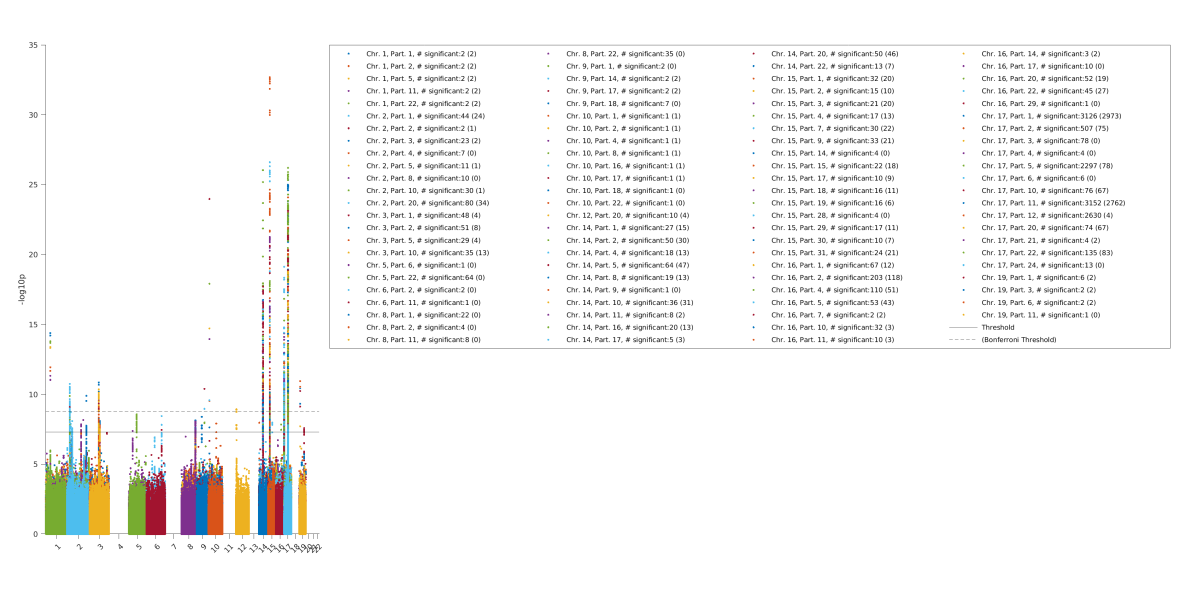
\includegraphics[width=\linewidth]{asymmetry/meta_analysis/joinedDatasets/mean_imputed/not_subsampled/partitions_gwas.pdf}
	\caption[Combined Manhattan plots across different partitions]{Combined Manhattan plots across different partitions, showing the number of significant \acp{snp} below the threshold of 5e-8 and with the Bonferroni correction, inside parentheses.}
	\label{fig:part_manhattan}


\end{adjustwidth}
\end{figure}
\chapter{Heritability}
\begin{figure}[H]
	\centering
\includesvg[width=0.5\textwidth]{asymmetry/visualizeHeritabilityOnPheno/joinedDatasets/mean_imputed/not_subsampled/Lambda GC.svg}
\caption[$\lambda_{GC}$ coefficient, as computed by LDSR]{$\lambda_{GC}$ coefficient, as computed by \ac{ldsr}. The observed $\chi^2$ value is close to the expected one at all studied partitions, with their ratio being close to 1.}	
\end{figure}
\chapter{Functional Analysis}
\begin{figure}[H]
	\centering
	\subfloat[Cell components]{
		\includegraphics[width=\textwidth]{asymmetry/FUMA gene2func/joinedDatasets/mean_imputed/not_subsampled/partitionsSummary/GO_CC.pdf}
	}
	\quad
	\subfloat[Biological processes]{
		\includegraphics[width=\textwidth]{asymmetry/FUMA gene2func/joinedDatasets/mean_imputed/not_subsampled/partitionsSummary/GO_BP.pdf}
	}
	\quad
	\subfloat[Molecular function]{
		\includegraphics[width=\textwidth]{asymmetry/FUMA gene2func/joinedDatasets/mean_imputed/not_subsampled/partitionsSummary/GO_MF.pdf}
	}
	\caption[GO terms enrichment analysis]{\Ac{go} terms enrichment analysis -log10 P-values (the higher value and the darker color, the more significant), as computed by FUMA, with the gene set augmented by GREAT.For all three cases, the entire hemisphere and the four 2nd level partition were assessed, however not all of the tests displayed a significant signal with \ac{go} terms.}
	\label{fig:go}
\end{figure}

\begin{figure}[H]
	\centering
	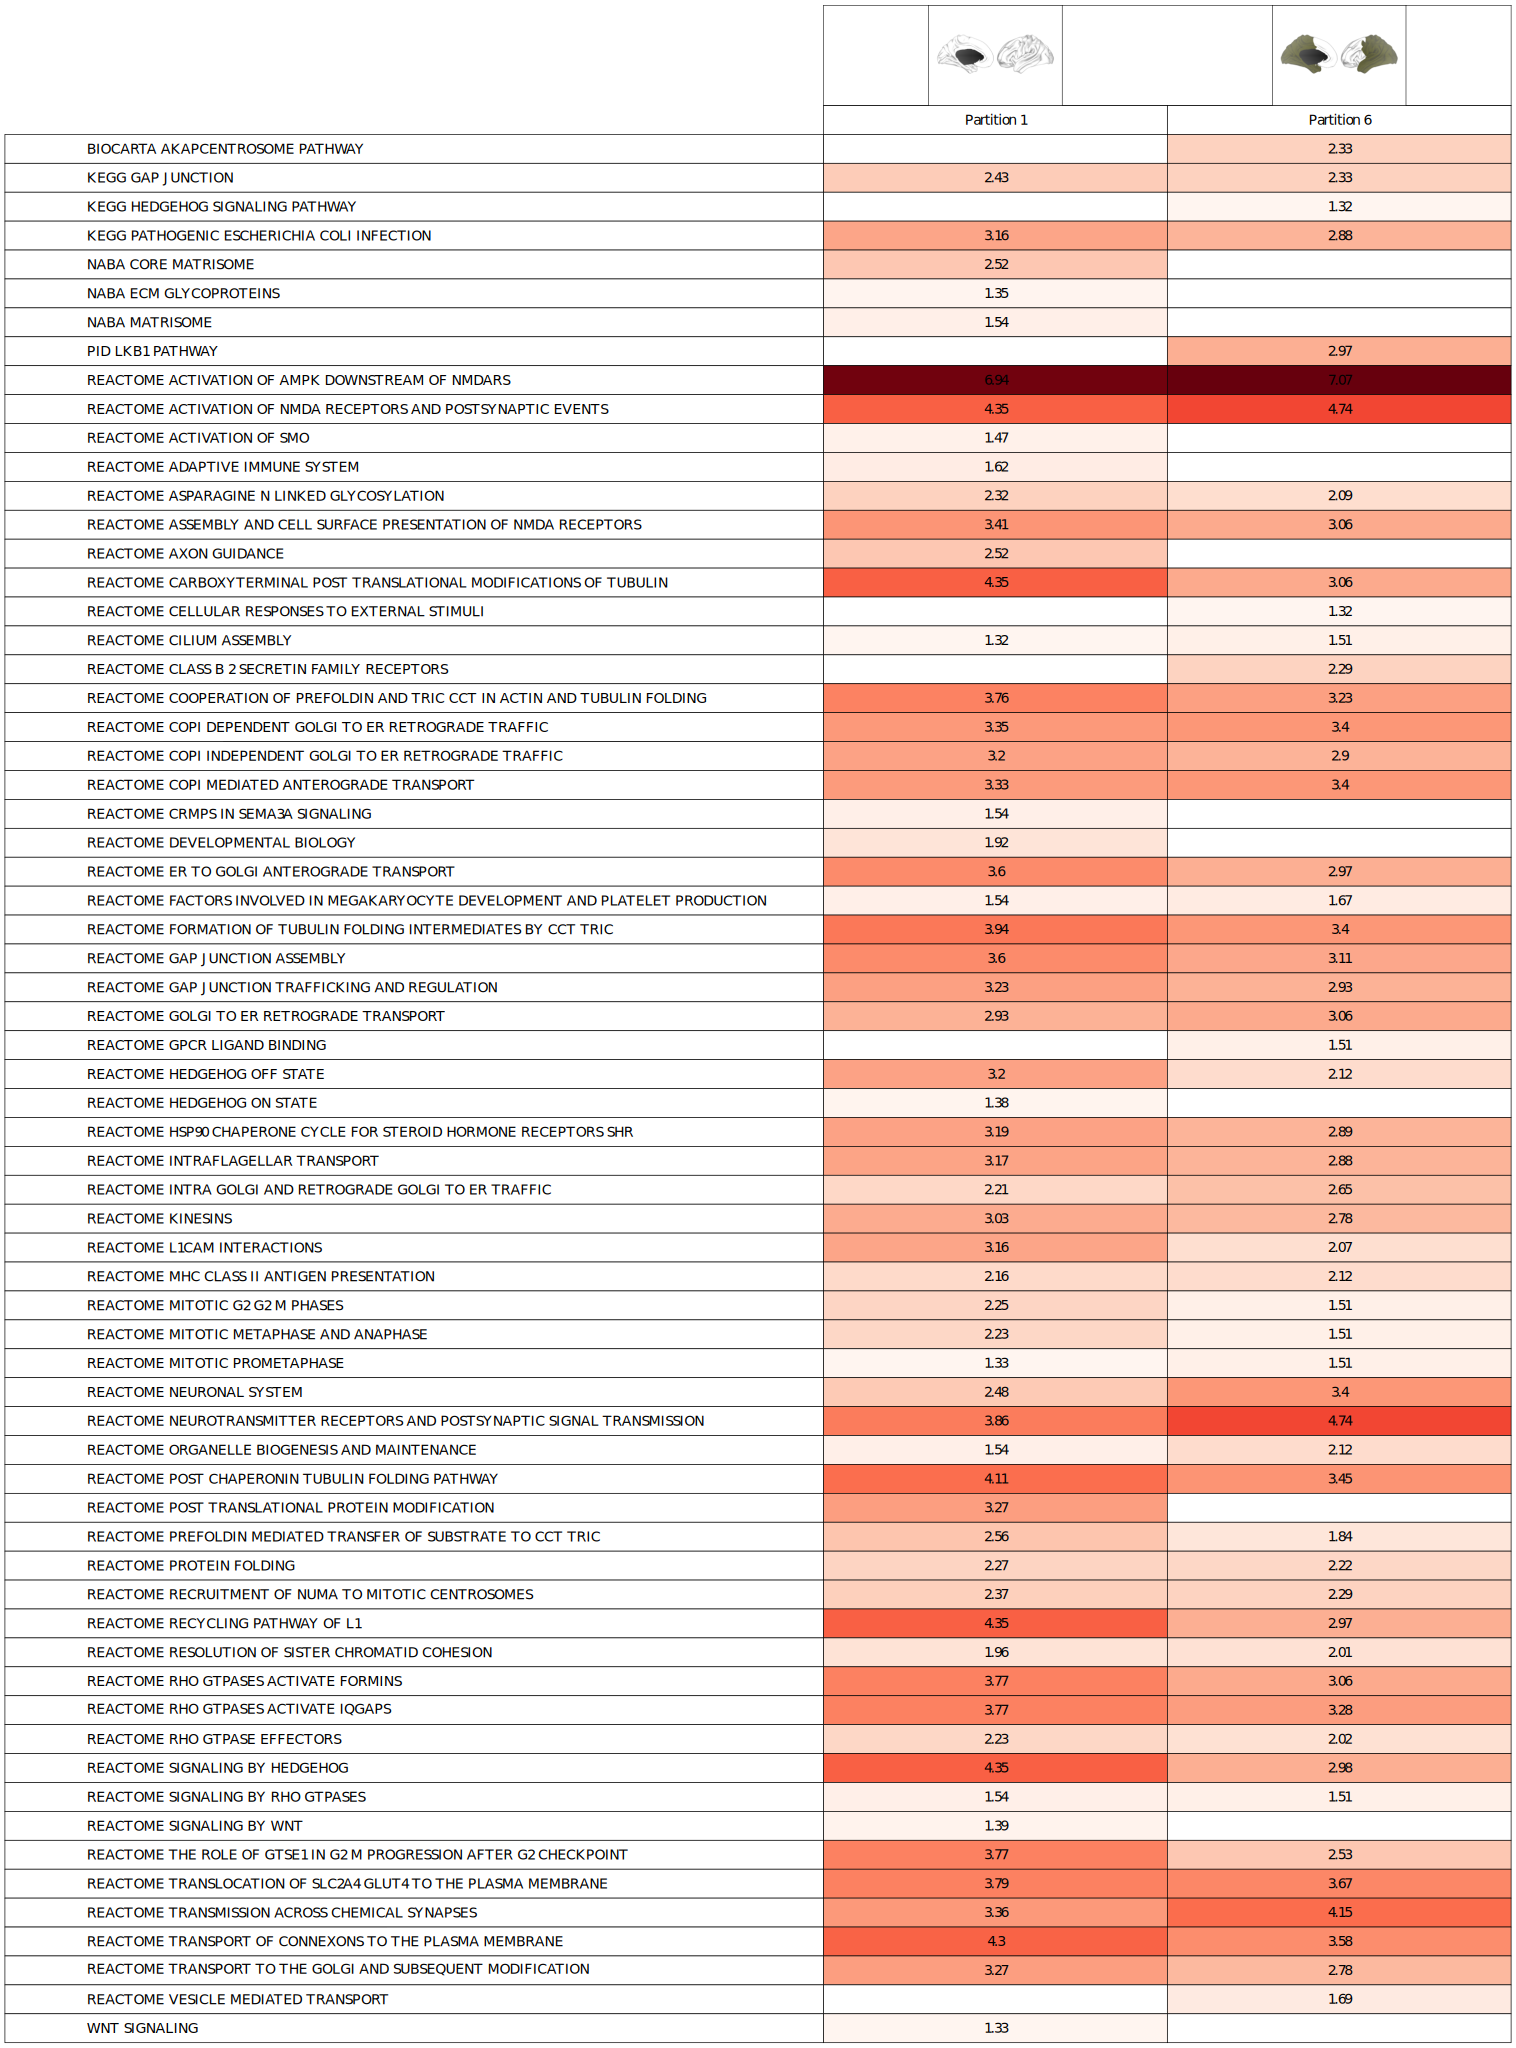
\includegraphics[width=\textwidth]{asymmetry/FUMA gene2func/joinedDatasets/mean_imputed/not_subsampled/partitionsSummary/canonical_pathways.pdf}
	
	\caption[Canonical pathways gene set enrichment analysis]{Differential gene set enrichment analysis performed on various canonical pathways reported by KEGG and Reactome, as computed by FUMA. Displayed -log10 P-values have increased lightness the higher the value.}
	\label{fig:can_pathways}
\end{figure}
\begin{figure}[H]
	\centering
	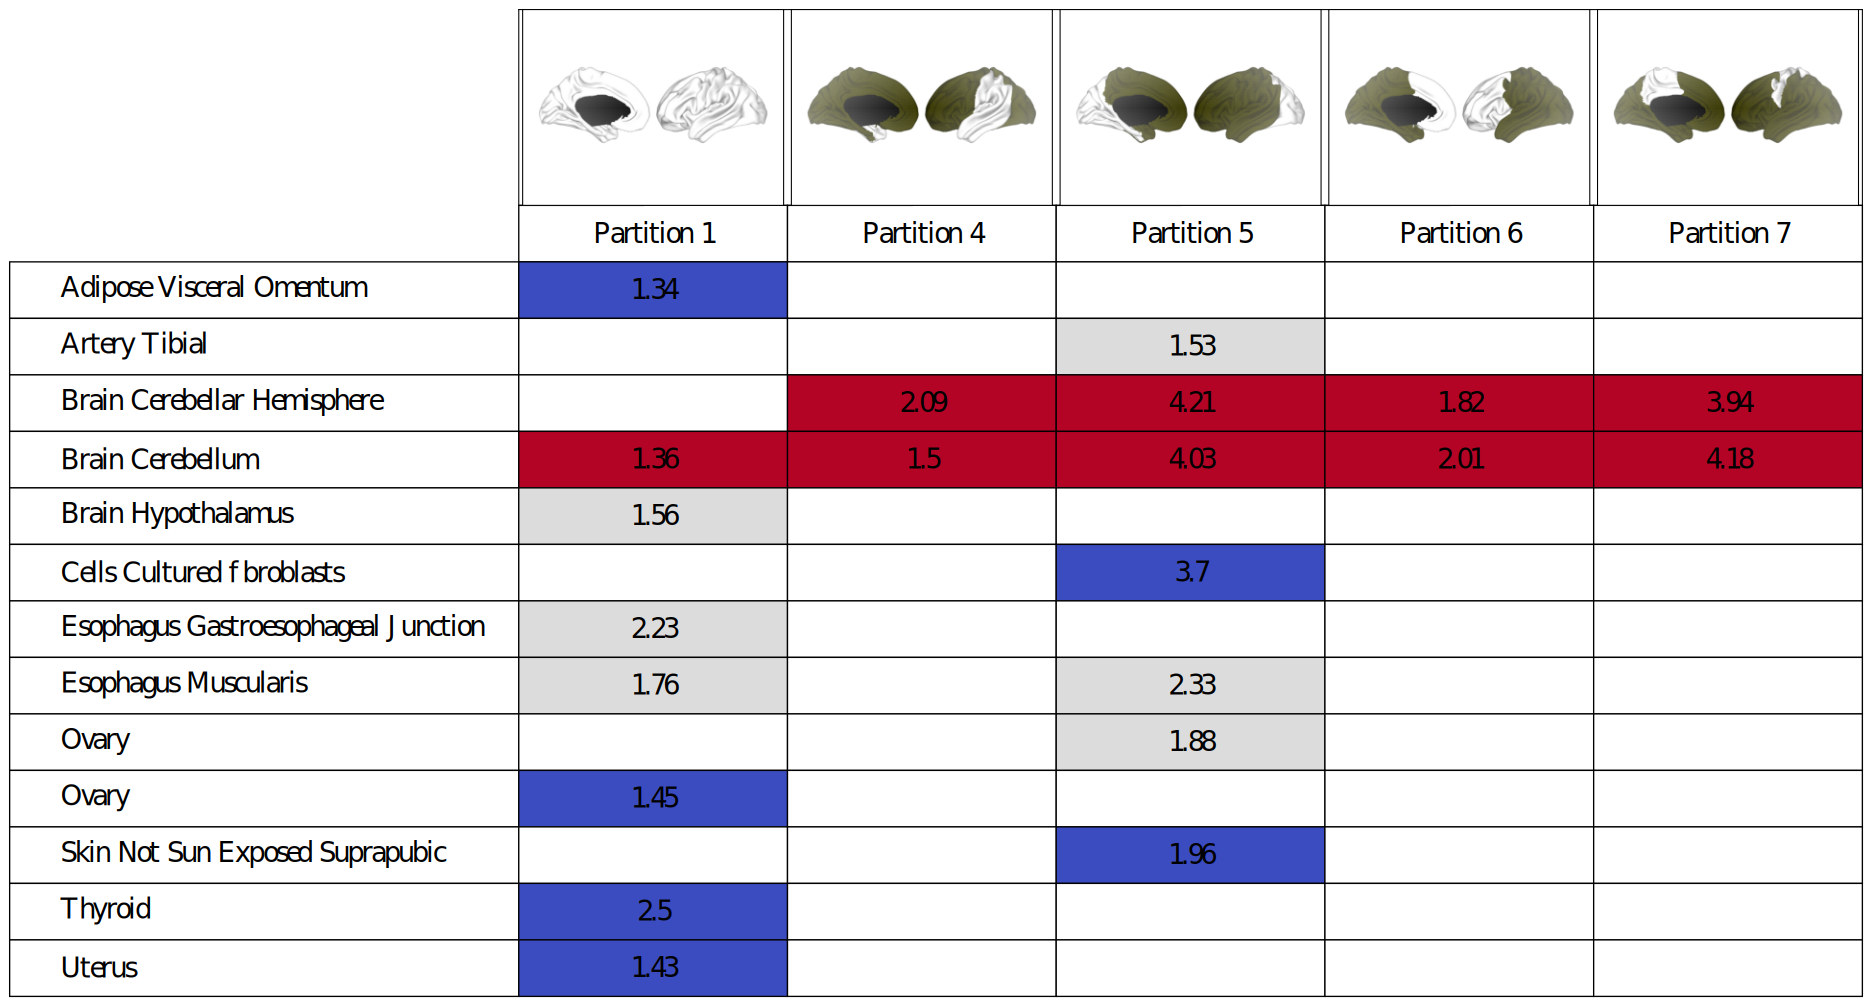
\includegraphics[width=\textwidth]{asymmetry/FUMA gene2func/joinedDatasets/mean_imputed/not_subsampled/partitionsSummary/DEG.pdf}
	
	\caption[Differential gene expression enrichment analysis]{Differential gene expression enrichment analysis performed on different tissues. Displayed -log10 P-values, as computed by FUMA using the identified partition-specific gene sets, are displayed in blue if the relation favors downregulated genes, red if it favors upregulated ones, or gray, if both downregulated and upregulated gene subsets are significantly enriched.}
	\label{fig:de_genes}
\end{figure}
\begin{figure}[H]
	\centering
	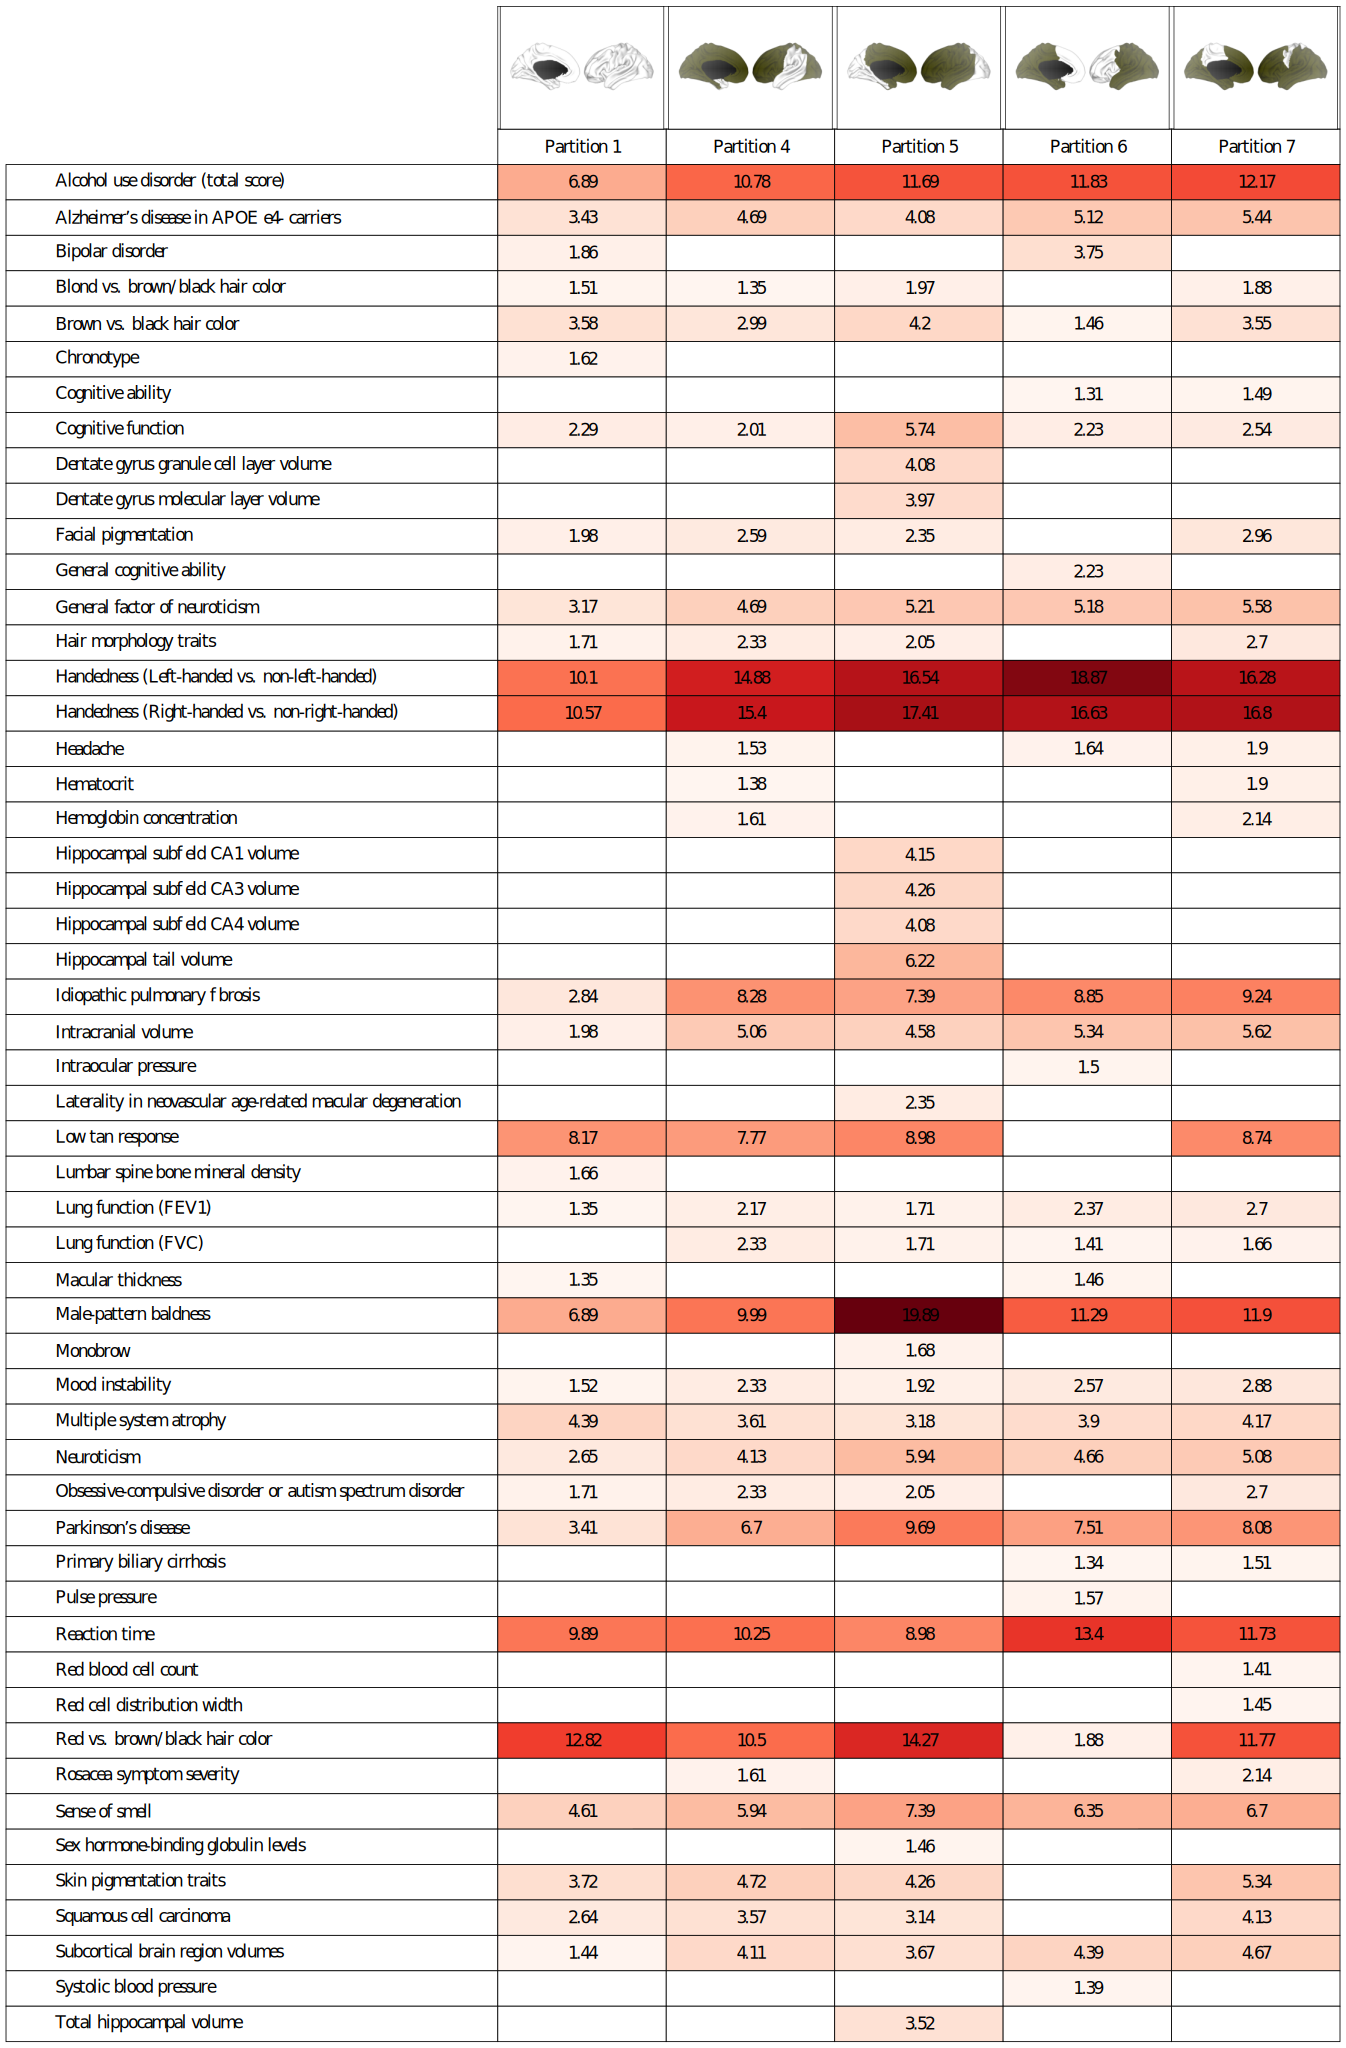
\includegraphics[width=\textwidth]{asymmetry/FUMA gene2func/joinedDatasets/mean_imputed/not_subsampled/partitionsSummary/GWASCatalog.pdf}
	
	\caption[GWAS Catalog gene set enrichment analysis]{Differential gene set enrichment analysis performed on various traits reported by GWAS catalog, as computed by FUMA. -log10 P-values are shown, with increased lightness the higher the value.}
	\label{fig:gw_catalog}
\end{figure}


\backmatter
\bibliographystyle{abbrv}
\bibliography{references}

\newenvironment{popsum}%
{\cleardoublepage\thispagestyle{empty}\null\vfill\begin{center}%
		\bfseries Popularized Summary\end{center}}%
{\vfill\null}
\begin{popsum}
The overall purpose of this thesis is to complement the existing bibliography on the detection and examination of the genetic associations of brain shape asymmetry.  Our body generally exhibits bilateral symmetry, namely our sides are mirrored images of each other. However, if someone pays close attention, not one feature is completely symmetric on each side of our body. In this thesis, we seek the genetic roots of this intrinsically complex trait, investigating the brain surface on healthy individuals of European origin from UK Biobank database. Cortical asymmetry has been found to be correlated with a variety of brain-related diseases, such as OCD, neuroticism and bipolar disorder,  and an early detection of the accountable genetic variants could be used for personalized diagnosis and treatment. Furthermore, brain asymmetry does not display the phenomenon of situs-inversus, that is internal organs occurring mirrored at certain individuals, which leads us to believe there is evolutionary pressure on this trait manifestation. Therefore, substantial heritability, namely phenotypic variation explained by genetic changes, is expected.

To this end, asymmetry statistical analysis was performed based on brain MRI scans, detecting regions with high affinity to display genetically inscribed asymmetry. A data-driven approach was then followed, where the brain surface was partitioned in multiple hierarchical levels, without any prior anatomic knowledge. Aggregated asymmetry measurements, retaining most of the included variation, were retrieved from the segments, whose genetic correlation was then examined through a multivariate genetic statistical analysis. Recognized significant variants were then compared against reported traits from other databases, based on monotonicity.  Functional annotations were constructed,  associating genetic variants to genes, offering an insight into the functional reasoning behind the brain shape asymmetry existence. The degree on which plasticity effect (that is the amount of variation not explained by the genome, but by  environmentally affected development) is dispersed throughout the brain was statistically mapped and genetically quantified, through genetic heritability studies. Novel causal region-specific genetic variants and increased heritability was identified throughout the entire hemisphere and the derived partitions, extending the related literature. Different spatially-dependent genetic profiles were identified. Connections with biological pathways, concerning intra- and extra-cellular organization and the formation of biological symmetry axes, were made, by examining protein-protein interactions. The effect of a strongly regulating, spatially dependent epigenetic effect on development was determined. Furthermore, gender-controlled epigenetic modifications appeared to affect cortical asymmetry. Lastly, associative studies led to the establishment of a tight, strongly supported, genetic bridge between  brain shape and asymmetry.
\end{popsum}
\end{document}